\documentclass[12pt,a4paper]{article}
\usepackage[utf8]{inputenc}
\usepackage[english,russian]{babel}
\usepackage{indentfirst}
\usepackage{misccorr}
\usepackage{graphicx}
\usepackage{amsmath}
\usepackage{latexsym}
\usepackage{cmap}
\usepackage{graphicx}



\begin{document}
\section{Теоретическое задание 4}
Рассмотрим смешанную краевую задачу с однородными граничными условиями для уравнения параболического типа:

\begin{equation*}
 \begin{cases}
   u_{t} = a^2 u_{xx} + f(x,t)
   \\
   u(x, 0) = \varphi(x)
   \\
   \alpha u(0, t) - \beta u_{x}(0, t) 
   = \gamma u(l, t) - \delta u_{x}(l,t) = 0
 \end{cases}
 \eqno(1)\
\end{equation*}

Решенеи задачи (1) имеет вид:

\begin{equation*}
  u(x, t) = \int\limits_0^l G(x, \xi, t) \varphi_{\varepsilon}(\xi)\,dx,
  \eqno(2)\
\end{equation*}

где

\begin{equation*}
   G(x, \xi, t) = \sum_{i=1}^\infty v_{n}(x) v_{n}(\xi).
  \eqno(3)\
\end{equation*}

\underline{Определение.} Функция $G(x, \xi, t)$, определяемая формулой (3) называется функцией Грина, или функцией влияния точечного источника.
\\
\\
Рассмотрим физический смысл функции Грина. В качестве начальной функции выберем непрерывную на отрезке $[0, l]$ функцию $\varphi_{\varepsilon}(x)$, равну $\Phi$ вне интервала (a, b), длинной $\alpha\epsilon$ с серединой в отрезке [0, l], и расположенную в этом интервале.

\begin{center}
\begin{equation*}
   \varphi_{\varepsilon}(x) \in C^0([0, l])
   \\
   (a, b) = K^{M_0}_{\varepsilon} \subset [0, l]
   \\
   \varphi_{\varepsilon}(x)|_{[0, l] \ (a, b)} = 0
\end{equation*}
\end{center}

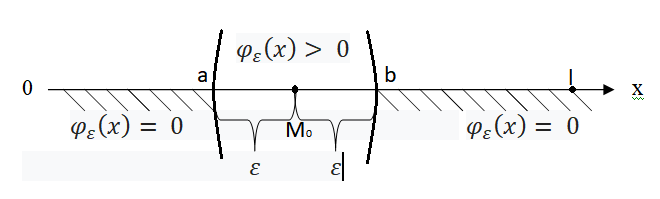
\includegraphics[scale=0.7]{pic1.png}

Пусть $\forall > 0$ функция $\varphi_{\epsilon}(x)$ удволетворяет условию нормировки:

\begin{center}
\begin{equation*}
   \int\limits_a^b \varphi_{\varepsilon}(x)\,dx = 1

\end{equation*}
\end{center}

Тогда,солгласно формуле (2), решение $u_{\epsilon}(x, t)$ задачи (1) с начальной функцией $\varphi_{\epsilon}(x)$ имеет вид:

\begin{equation*}
   u_{\epsilon}(x, t)
   = \int\limits_0^l G(x, \xi, t) \varphi_{\varepsilon}(\xi)\,dx
   = \int\limits_a^b G(x, \xi, t) \varphi_{\varepsilon}(\xi)\,dx 
\end{equation*}

Далее, согласно первой формуле среднего значения в обобщенной форму, \exists M^*:

\begin{equation*}
   \int\limits_a^b G(x, \xi, t) \varphi_{\varepsilon}(\xi)\,dx
   = G(x, M^*, t) \int\limits_a^b \varphi_{\varepsilon}(\xi)\,dx 
   = G(x, M^*, t)
   \eqno(4)\
\end{equation*}

Перейдя в формуле (4) к пределу по $\epsilon \to 0$, получилм:

\begin{equation*}
   u_{0}(x, t) = \lim_{\epsilon \to 0} u_{\epsilon}(x, t)
   = \lim_{\epsilon \to 0} G(x, M^*, t)
   = G(x, M_{0}, t)
   \eqno(5)\
\end{equation*}

Из формулы (5) следует, что функция Грина с физической точки зрения, представляет собой температуру тела в момент времени $t$ в точке $x$, если возбуждение тела производится мгновенным точечным источником, действущим мощностью в момент времени $t = 0$ вточке $M_{0}$.
\\
\\
Найдем мощность точечного источника.
Количество тепла q, сообщенное телу в начальный момент времени $t = 0$, равно:

\begin{center}
\begin{equation*}
   q = \lim_{\epsilon \to 0} \int\limits_0^l c \rho  \varphi_{\epsilon}(\xi)
   = \lim_{\epsilon \to 0} \int\limits_0^l \varphi_{\epsilon}(\xi) 
   = \lim_{\epsilon \to 0} \int\limits_a^b \varphi_{\epsilon}(\xi) = 1
   \eqno(6)\
\end{equation*}
\end{center}

Таким образом, функция Грина $G(x, M_{0}, t)$ есть температура тела в точке $x$ в момент времени $t$ при мгновенном выделении единичного (см. формулу (6)) количество тепла в точке $M_0$ в момент времени $t = 0$. 

\end{document}